\documentclass{standalone}
\usepackage{tikz}
\usetikzlibrary{patterns}
\usetikzlibrary{positioning}
\usetikzlibrary{patterns, positioning}
\usetikzlibrary{shapes.misc}
\usepackage[outline]{contour}
\contourlength{1.5pt} 
\usepackage[sfdefault]{ClearSans}

\begin{document}
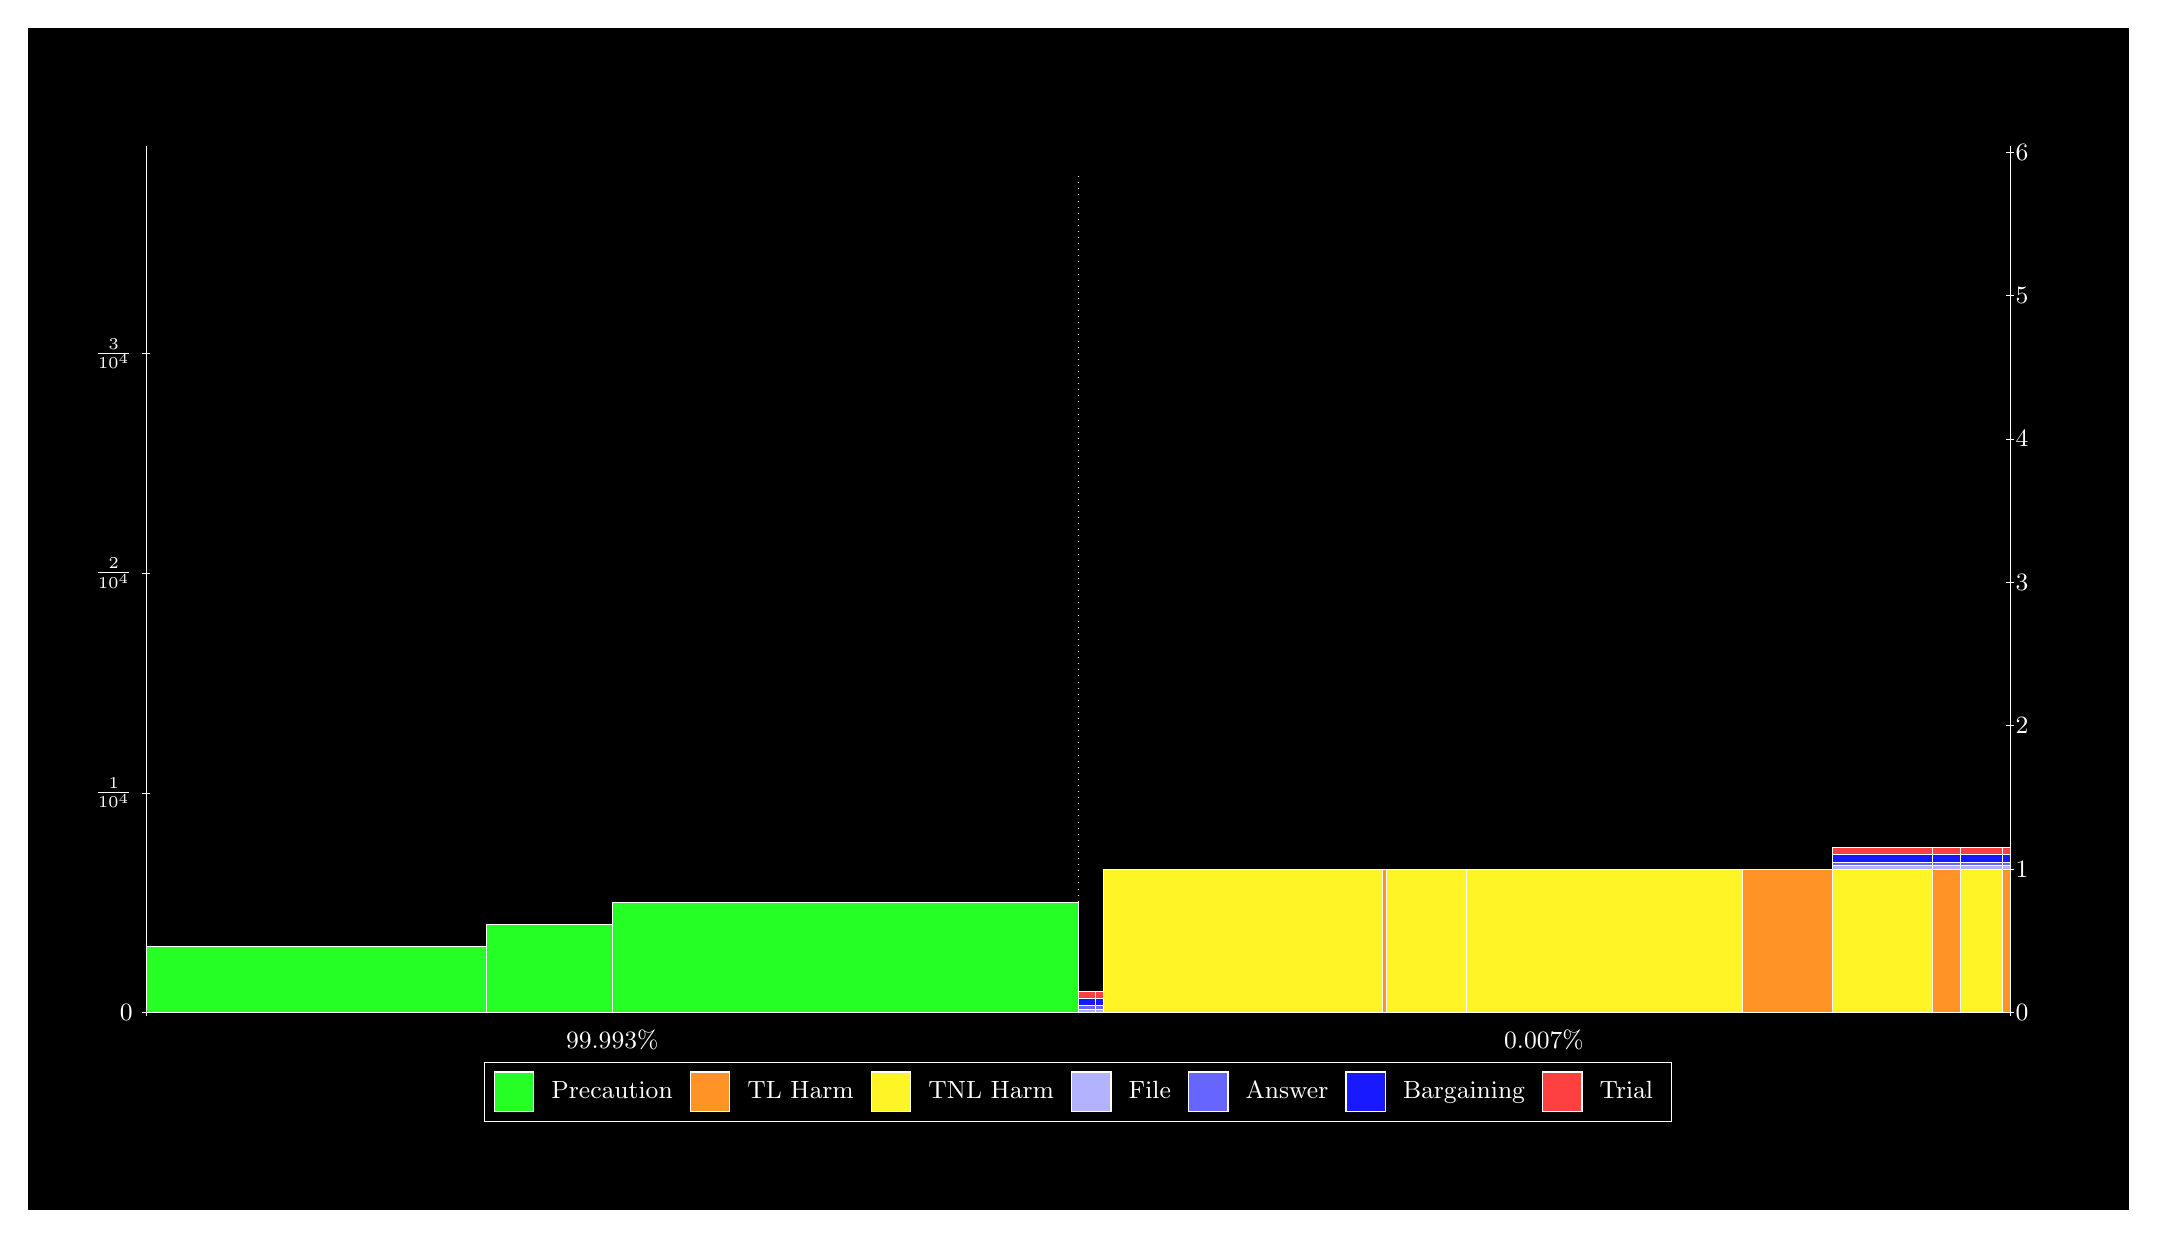
\begin{tikzpicture}
\draw[fill=black] (0,0) rectangle (26.667,15);
\draw[fill=green!85,draw=white,very thin] (1.5,2.5) rectangle (5.8205,3.3369);
\draw[fill=green!85,draw=white,very thin] (5.8205,2.5) rectangle (7.4166,3.6159);
\draw[fill=green!85,draw=white,very thin] (7.4166,2.5) rectangle (13.333,3.8948);
\draw[fill=green!85,draw=white,very thin] (13.333,2.5) rectangle (13.548,2.5001);
\draw[fill=blue!30,draw=white,very thin] (13.333,2.5001) rectangle (13.548,2.5456);
\draw[fill=blue!60,draw=white,very thin] (13.333,2.5456) rectangle (13.548,2.5911);
\draw[fill=blue!90,draw=white,very thin] (13.333,2.5911) rectangle (13.548,2.6822);
\draw[fill=red!75,draw=white,very thin] (13.333,2.6822) rectangle (13.548,2.7732);
\draw[fill=green!85,draw=white,very thin] (13.548,2.5) rectangle (13.649,2.5001);
\draw[fill=blue!30,draw=white,very thin] (13.548,2.5001) rectangle (13.649,2.5456);
\draw[fill=blue!60,draw=white,very thin] (13.548,2.5456) rectangle (13.649,2.5911);
\draw[fill=blue!90,draw=white,very thin] (13.548,2.5911) rectangle (13.649,2.6822);
\draw[fill=red!75,draw=white,very thin] (13.548,2.6822) rectangle (13.649,2.7732);
\draw[fill=green!85,draw=white,very thin] (13.649,2.5) rectangle (17.202,2.5001);
\draw[fill=yellow!85,draw=white,very thin] (13.649,2.5001) rectangle (17.202,4.3211);
\draw[fill=green!85,draw=white,very thin] (17.202,2.5) rectangle (17.25,2.5001);
\draw[fill=orange!85,draw=white,very thin] (17.202,2.5001) rectangle (17.25,4.3211);
\draw[fill=green!85,draw=white,very thin] (17.25,2.5) rectangle (18.261,2.5001);
\draw[fill=yellow!85,draw=white,very thin] (17.25,2.5001) rectangle (18.261,4.3212);
\draw[fill=green!85,draw=white,very thin] (18.261,2.5) rectangle (18.266,2.5001);
\draw[fill=orange!85,draw=white,very thin] (18.261,2.5001) rectangle (18.266,4.3212);
\draw[fill=green!85,draw=white,very thin] (18.266,2.5) rectangle (21.772,2.5001);
\draw[fill=yellow!85,draw=white,very thin] (18.266,2.5001) rectangle (21.772,4.3212);
\draw[fill=green!85,draw=white,very thin] (21.772,2.5) rectangle (22.914,2.5001);
\draw[fill=orange!85,draw=white,very thin] (21.772,2.5001) rectangle (22.914,4.3212);
\draw[fill=green!85,draw=white,very thin] (22.914,2.5) rectangle (24.178,2.5001);
\draw[fill=yellow!85,draw=white,very thin] (22.914,2.5001) rectangle (24.178,4.3211);
\draw[fill=blue!30,draw=white,very thin] (22.914,4.3211) rectangle (24.178,4.3667);
\draw[fill=blue!60,draw=white,very thin] (22.914,4.3667) rectangle (24.178,4.4122);
\draw[fill=blue!90,draw=white,very thin] (22.914,4.4122) rectangle (24.178,4.5032);
\draw[fill=red!75,draw=white,very thin] (22.914,4.5032) rectangle (24.178,4.5943);
\draw[fill=green!85,draw=white,very thin] (24.178,2.5) rectangle (24.538,2.5001);
\draw[fill=orange!85,draw=white,very thin] (24.178,2.5001) rectangle (24.538,4.3211);
\draw[fill=blue!30,draw=white,very thin] (24.178,4.3211) rectangle (24.538,4.3667);
\draw[fill=blue!60,draw=white,very thin] (24.178,4.3667) rectangle (24.538,4.4122);
\draw[fill=blue!90,draw=white,very thin] (24.178,4.4122) rectangle (24.538,4.5032);
\draw[fill=red!75,draw=white,very thin] (24.178,4.5032) rectangle (24.538,4.5943);
\draw[fill=green!85,draw=white,very thin] (24.538,2.5) rectangle (25.071,2.5001);
\draw[fill=yellow!85,draw=white,very thin] (24.538,2.5001) rectangle (25.071,4.3212);
\draw[fill=blue!30,draw=white,very thin] (24.538,4.3212) rectangle (25.071,4.3667);
\draw[fill=blue!60,draw=white,very thin] (24.538,4.3667) rectangle (25.071,4.4122);
\draw[fill=blue!90,draw=white,very thin] (24.538,4.4122) rectangle (25.071,4.5033);
\draw[fill=red!75,draw=white,very thin] (24.538,4.5033) rectangle (25.071,4.5943);
\draw[fill=green!85,draw=white,very thin] (25.071,2.5) rectangle (25.167,2.5001);
\draw[fill=orange!85,draw=white,very thin] (25.071,2.5001) rectangle (25.167,4.3212);
\draw[fill=blue!30,draw=white,very thin] (25.071,4.3212) rectangle (25.167,4.3667);
\draw[fill=blue!60,draw=white,very thin] (25.071,4.3667) rectangle (25.167,4.4122);
\draw[fill=blue!90,draw=white,very thin] (25.071,4.4122) rectangle (25.167,4.5033);
\draw[fill=red!75,draw=white,very thin] (25.071,4.5033) rectangle (25.167,4.5943);
\draw[white,very thin] (1.5,2.5) -- (1.5,13.5);
\draw[white,very thin] (1.45,2.5) -- (1.55,2.5);
\node[font=\small,text=white, anchor=east] at (1.45, 2.5) {0};
\draw[white,very thin] (1.45,5.2897) -- (1.55,5.2897);
\node[font=\small,text=white, anchor=east] at (1.45, 5.2897) {$\frac{1}{10^{4}}$};
\draw[white,very thin] (1.45,8.0794) -- (1.55,8.0794);
\node[font=\small,text=white, anchor=east] at (1.45, 8.0794) {$\frac{2}{10^{4}}$};
\draw[white,very thin] (1.45,10.869) -- (1.55,10.869);
\node[font=\small,text=white, anchor=east] at (1.45, 10.869) {$\frac{3}{10^{4}}$};

\draw[white,dotted,very thin] (13.333,2.83) -- (13.333,13.17);
\draw[white,very thin] (25.167,2.5) -- (25.167,13.5);
\draw[white,very thin] (25.117,2.5) -- (25.217,2.5);
\node[font=\small,text=white, anchor=west] at (25.117, 2.5) {0};
\draw[white,very thin] (25.117,4.3211) -- (25.217,4.3211);
\node[font=\small,text=white, anchor=west] at (25.117, 4.3211) {1};
\draw[white,very thin] (25.117,6.1422) -- (25.217,6.1422);
\node[font=\small,text=white, anchor=west] at (25.117, 6.1422) {2};
\draw[white,very thin] (25.117,7.9632) -- (25.217,7.9632);
\node[font=\small,text=white, anchor=west] at (25.117, 7.9632) {3};
\draw[white,very thin] (25.117,9.7843) -- (25.217,9.7843);
\node[font=\small,text=white, anchor=west] at (25.117, 9.7843) {4};
\draw[white,very thin] (25.117,11.605) -- (25.217,11.605);
\node[font=\small,text=white, anchor=west] at (25.117, 11.605) {5};
\draw[white,very thin] (25.117,13.426) -- (25.217,13.426);
\node[font=\small,text=white, anchor=west] at (25.117, 13.426) {6};

\draw[white,very thin] (1.5,2.5) -- (25.167,2.5);
\draw[white,very thin] (1.5,2.45) -- (1.5,2.55);
\node[font=\small,text=white, anchor=north] at (1.5, 2.45) {};
\draw[white,very thin] (25.167,2.45) -- (25.167,2.55);
\node[font=\small,text=white, anchor=north] at (25.167, 2.45) {};

\node[font=\small,text=white,anchor=south] at (7.4167, 1.9) {99.993\%};
\node[font=\small,text=white,anchor=south] at (19.25, 1.9) {0.007\%};
\draw (13.3333,2.5) node (B) {};
\begin{scope}[align=center]
\matrix[scale=0.5,draw=white,below=0.5cm of B,nodes={draw},column sep=0.1cm]{
\node[rectangle,draw,minimum width=0.5cm,minimum height=0.5cm,fill=green!85]{}; & \node[draw=none,font=\small,text=white]{Precaution}; &
\node[rectangle,draw,minimum width=0.5cm,minimum height=0.5cm,fill=orange!85]{}; & \node[draw=none,font=\small,text=white]{TL Harm}; &
\node[rectangle,draw,minimum width=0.5cm,minimum height=0.5cm,fill=yellow!85]{}; & \node[draw=none,font=\small,text=white]{TNL Harm}; &
\node[rectangle,draw,minimum width=0.5cm,minimum height=0.5cm,fill=blue!30]{}; & \node[draw=none,font=\small,text=white]{File}; &
\node[rectangle,draw,minimum width=0.5cm,minimum height=0.5cm,fill=blue!60]{}; & \node[draw=none,font=\small,text=white]{Answer}; &
\node[rectangle,draw,minimum width=0.5cm,minimum height=0.5cm,fill=blue!90]{}; & \node[draw=none,font=\small,text=white]{Bargaining}; &
\node[rectangle,draw,minimum width=0.5cm,minimum height=0.5cm,fill=red!75]{}; & \node[draw=none,font=\small,text=white]{Trial}; \\\\
};\end{scope}

\end{tikzpicture}
\end{document}